\chapter{Results}
\label{chap:results}

In this section, the results from the proposed solution is described in detail. It describes different results from the different stages throughout the develop process and presents the final results and metrics from the trained \acrfull{ml} model.

\section{Constructed dataset and ML problem formulation}

The initial dataset was copied and validated from \acrfull{mo}'s \acrshort{ais} database. The database table \textit{``vessel\_positions\_history''} was last updated in March 2021 and consists of \textbf{1.2} billion positional \acrshort{ais} records. Each vessel that transmitted positions belongs to a given segment and sub-segment that was made available by the \textit{``vessel\_segment''} table which contains \textbf{eight} different segment values, and \textbf{107} different combinations of segments and sub-segments. The provided \textit{``ports''} data contains \textbf{5200} ports world-wide that all follows the \gls{locode} naming standard. In total, as of March 2021, there were \textbf{6.4} million vessel transitions in the \textit{``vessel\_transitions''} table which was used to construct voyages. This data formed the initial data foundation for the final processed \acrfull{ml} training dataset. All the data that was copied and processed from \acrshort{mo}'s databases were processed in batches. Ports, segments, and transitions where quickly copied and processed, however, the \textbf{1.2} billion positional records took several days to migrate and validate. This was mostly because of the time required to validate coordinates and correctly map \acrshort{mmsi} and \acrshort{imo} values. Throughout this process, the latest identifiers and timestamps were fetched from the dedicated project database to only update data that occurred after the latest records already processed. In this way, this process was idempotent so that running the process multiple times did not affect existing data. This made the system simple to update throughout the development process and as many records as possible were used in the final approach only limited by the thesis time limitation.

\subsection{Voyage definition and construction}
\label{sec:results_voyage_definition}

Based on the initial \textbf{6.4} million vessel transitions, \textbf{1.7} million voyages where initially constructed by finding positional records transmitted from a vessel between subsequent departure and arrival transitions. The resulting voyages were, therefore, defined based on transitioning \acrshort{ais} statuses that indicate the vessel is moored or moving. As a consequence of this definition, the quality of the resulting trajectories are very much affected by how well the \gls{aivdm} protocol is followed by the traveling vessels. Since the navigational status attribute is manually inputted by the vessel's captain or crew, the resulting trajectories are prone to human error but results in more complete voyages disregarding intermediate stops for purposes such as bunkering.

As an example, \cref{fig:transition_voyage} shows a voyage from China to Argentina where the vessel stopped at Singapore, most likely to bunker. In the chosen voyage definition, the beginning and end of the voyage is defined based on input from the vessel's captain which results in a voyage starting from China, and ending in Argentina. Further implications and consequences of the chosen definition is later discussed in \cref{chap:discussion}.

\begin{figure}[htbp]
    \centering
    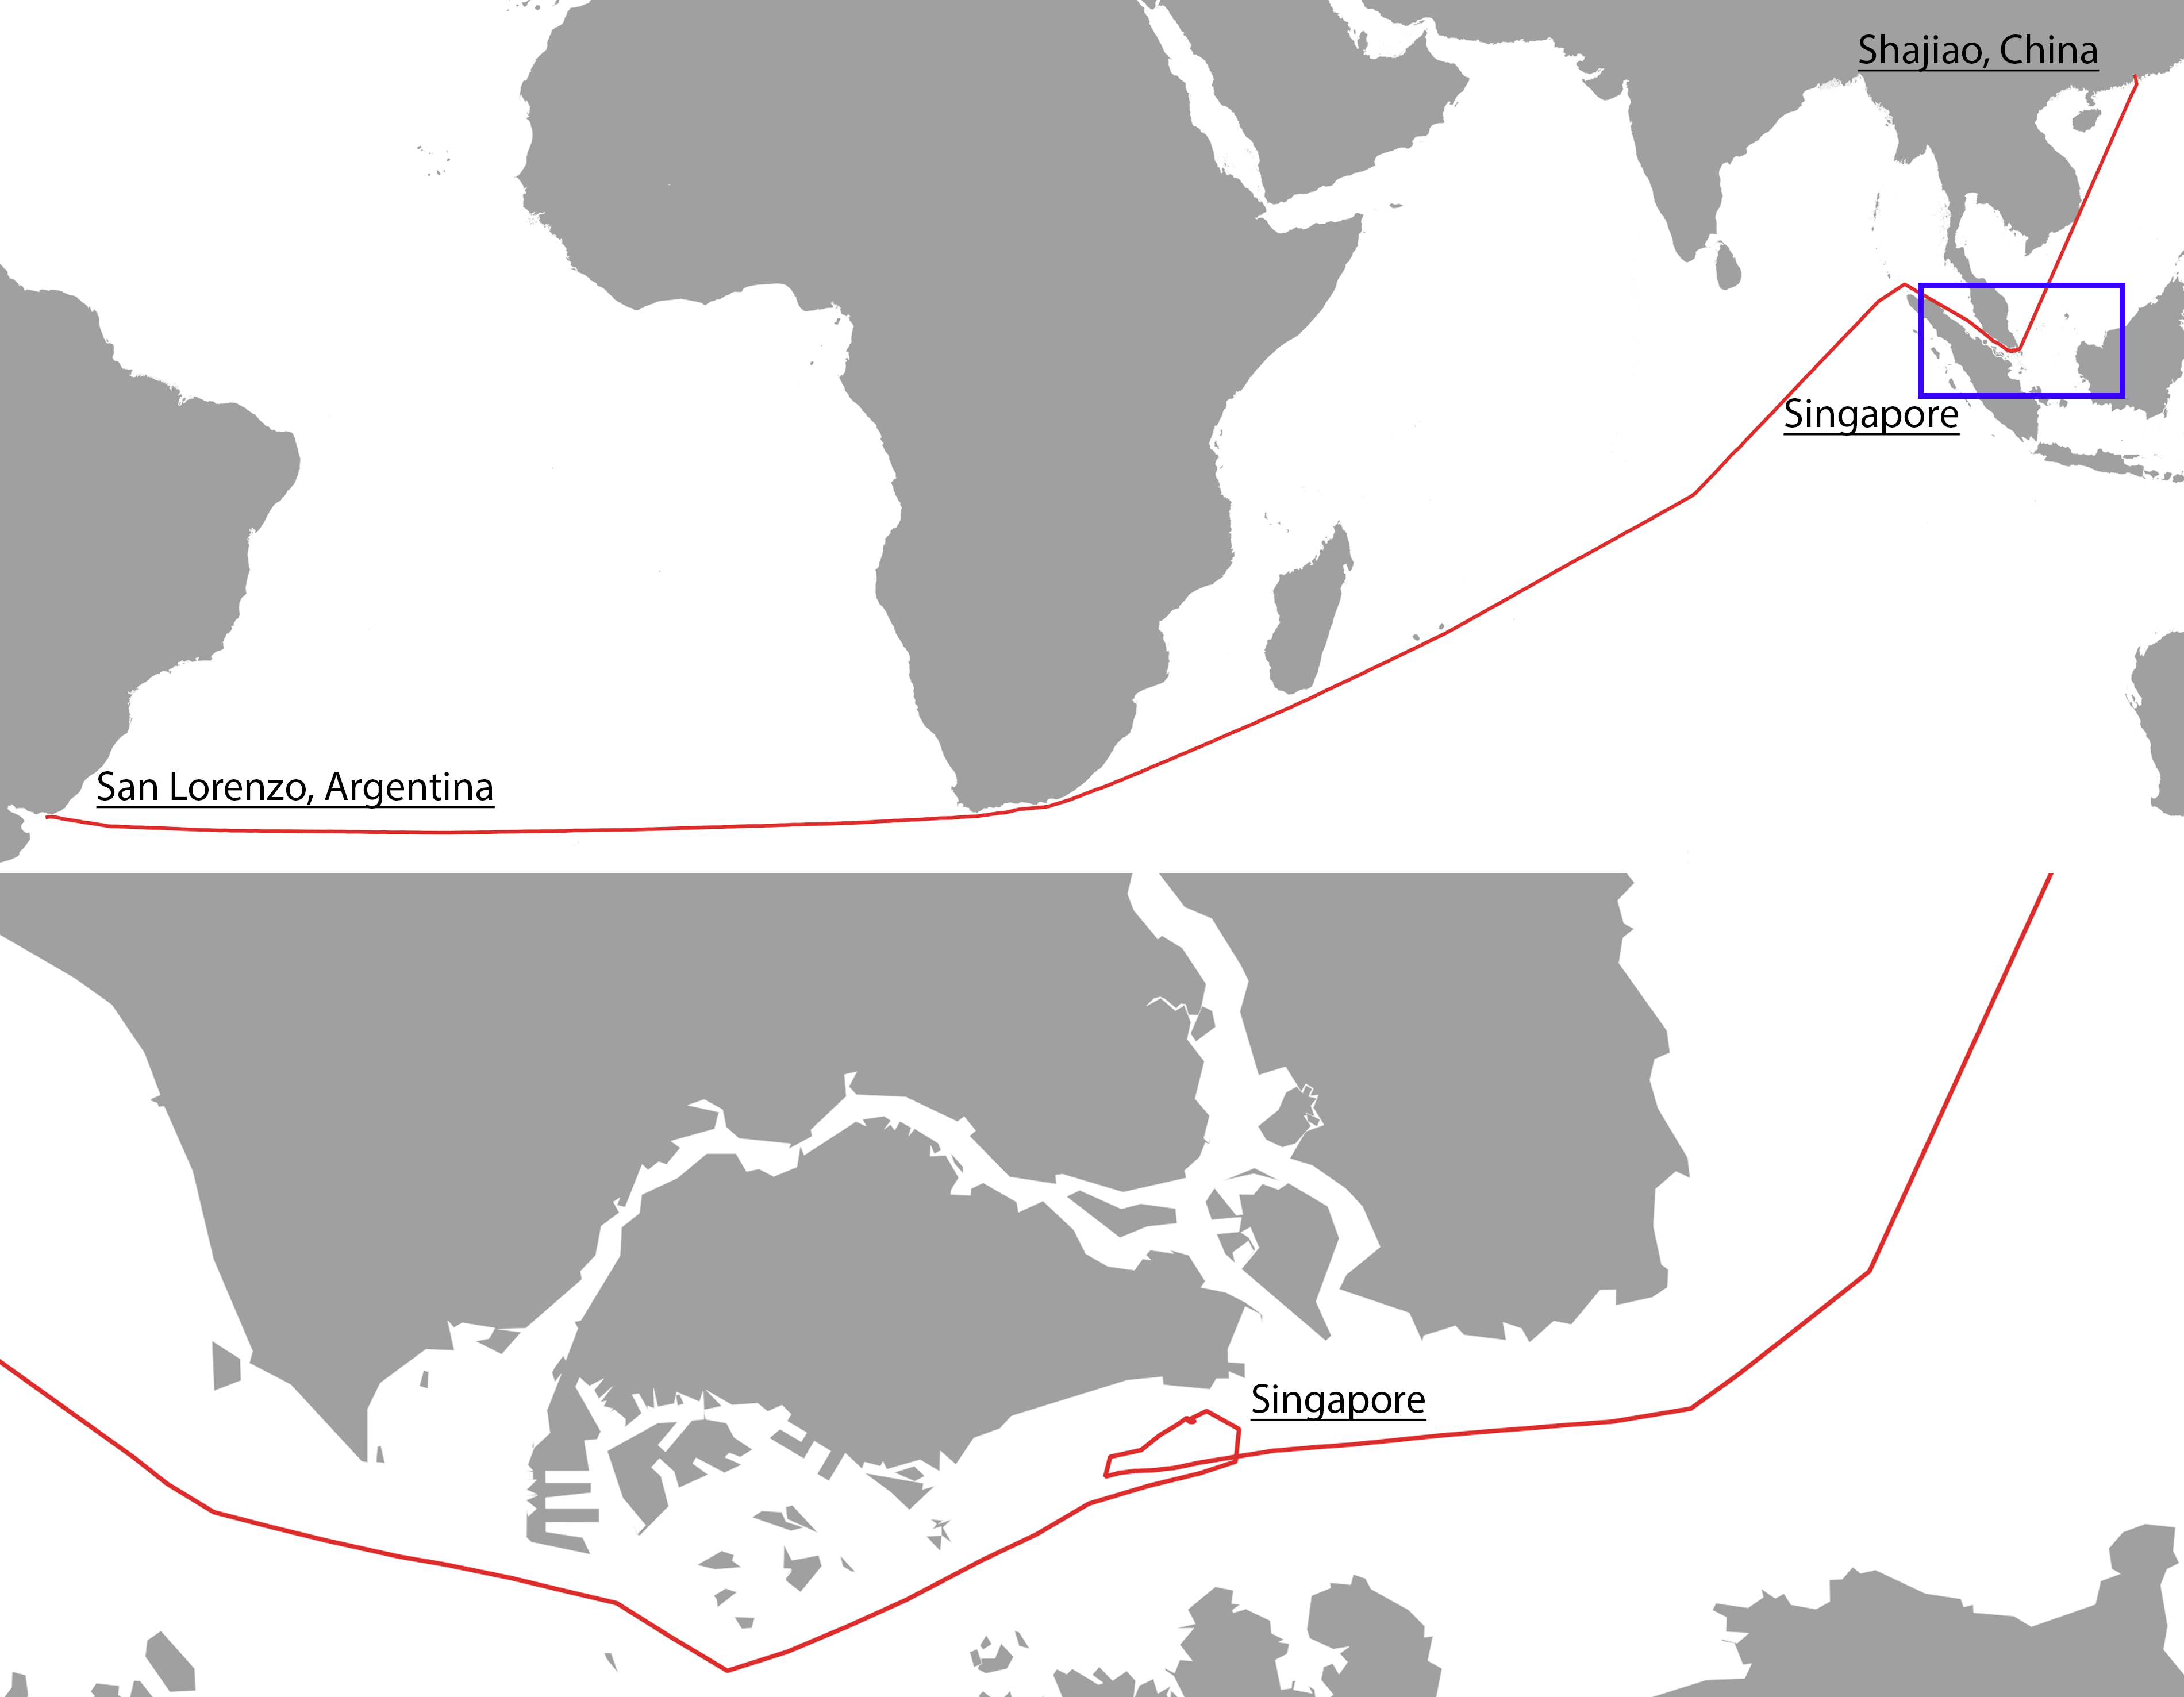
\includegraphics[width=1.0\textwidth]{figures/results/voyage_quality}
    \caption{Transition voyage from China to Argentina that visits the port of Singapore exemplifying the properties of the chosen voyage definition.}
    \label{fig:transition_voyage}
\end{figure}

The \textbf{1.7} million voyages constructed using the vessel transitions were sampled based on 6 hour intervals and collected in ``sampled\_transition\_voyages'' that formed the foundation for trajectory similarity measurements. In the process of constructing the final dataset, these sampled voyages were divided into multiple incomplete voyages up to a factor of four. The resulting training dataset collected in the table ``ml\_training\_data'' consisted of \textbf{4.3} million voyages.

\subsection{Trajectory similarity and MSTD}

Using the foundation of the sampled trajectories, each trajectory was compared to every other trajectory departing the same port to calculate the \acrfull{mstd}. The \acrshort{mstd} value was used primarily as a method of abstracting geographical trajectories into categorical and numerical values that a \acrfull{ml} model could work with. This process converted a voyage's geographical trajectory into MSTD, the similarity value to the most similar trajectory, and trajectory length. Thus, the MSTD value served as an initial prediction purely based on geographical trajectory similarity measurements using \acrfull{sspd}. The \acrshort{sspd} method was chosen for its ability to effectively handle different lengths and shapes of trajectories when estimating similarity. Furthermore, in the approach proposed in \cite{Zhang2020AISApproach} the \acrshort{sspd} method performed the best out of the algorithmic approaches evaluated, although, their own Random Forest (RF) based approach performed the best. However, the way the training data is structured, the trajectory similarity method of choice is completely interchangeable with others. The only requirement for a given trajectory similarity measurement is that it also produces a similarity value that serves as a weight for the \acrshort{mstd} value.

\acrshort{mstd} as an initial prediction seemed to be a decent initial indicator as to where the vessel would be arriving. In total, there were \textbf{4 306 271} entries in the final training data generated where exactly \textbf{1 423 476} of which has the same arrival port and \acrshort{mstd} value. Thus, it can be assumed that the purely spatial prediction using incomplete sampled historical voyages based on \acrshort{sspd} was \textit{33\%} accurate. In other words, when using an algorithmic prediction approach based on purely spatial trajectory similarity measurements, voyage destinations can be predicted correctly one third of the time. This formed a baseline accuracy to beat with the \acrshort{ml}-based solution.

\subsection{ML data preparation}

After the final training dataset was built, it was discovered that in terms of arrival port frequencies, the dataset was imbalanced thus making it harder for \acrshort{ml} models to learn. Although some models can better handle dataset imbalance, a sampling approach was used to balance the dataset before training to support different ML models. Several different sampling approaches were evaluated, however, the traditional over and under -sampling methods either produced massive amounts of synthetic data, or removed almost all the original data which was shown in \cref{fig:all_samplers} in \cref{chap:method}. Thus, an ensemble sampling method of majority undersampling and ``SMOTE+ENN'' was employed to balance the dataset before training. \cref{fig:ensemble_sampler} shows the results from the ensemble sampling method that uses a combination of under and over -sampling techniques. As \cref{fig:ensemble_sampler} shows, using a subset of the full dataset, the final result is 8\% smaller than the original dataset, is a lot more balanced, but still has differences in class frequencies which persisted from the original dataset.

\begin{figure}[htbp]
    \centering
    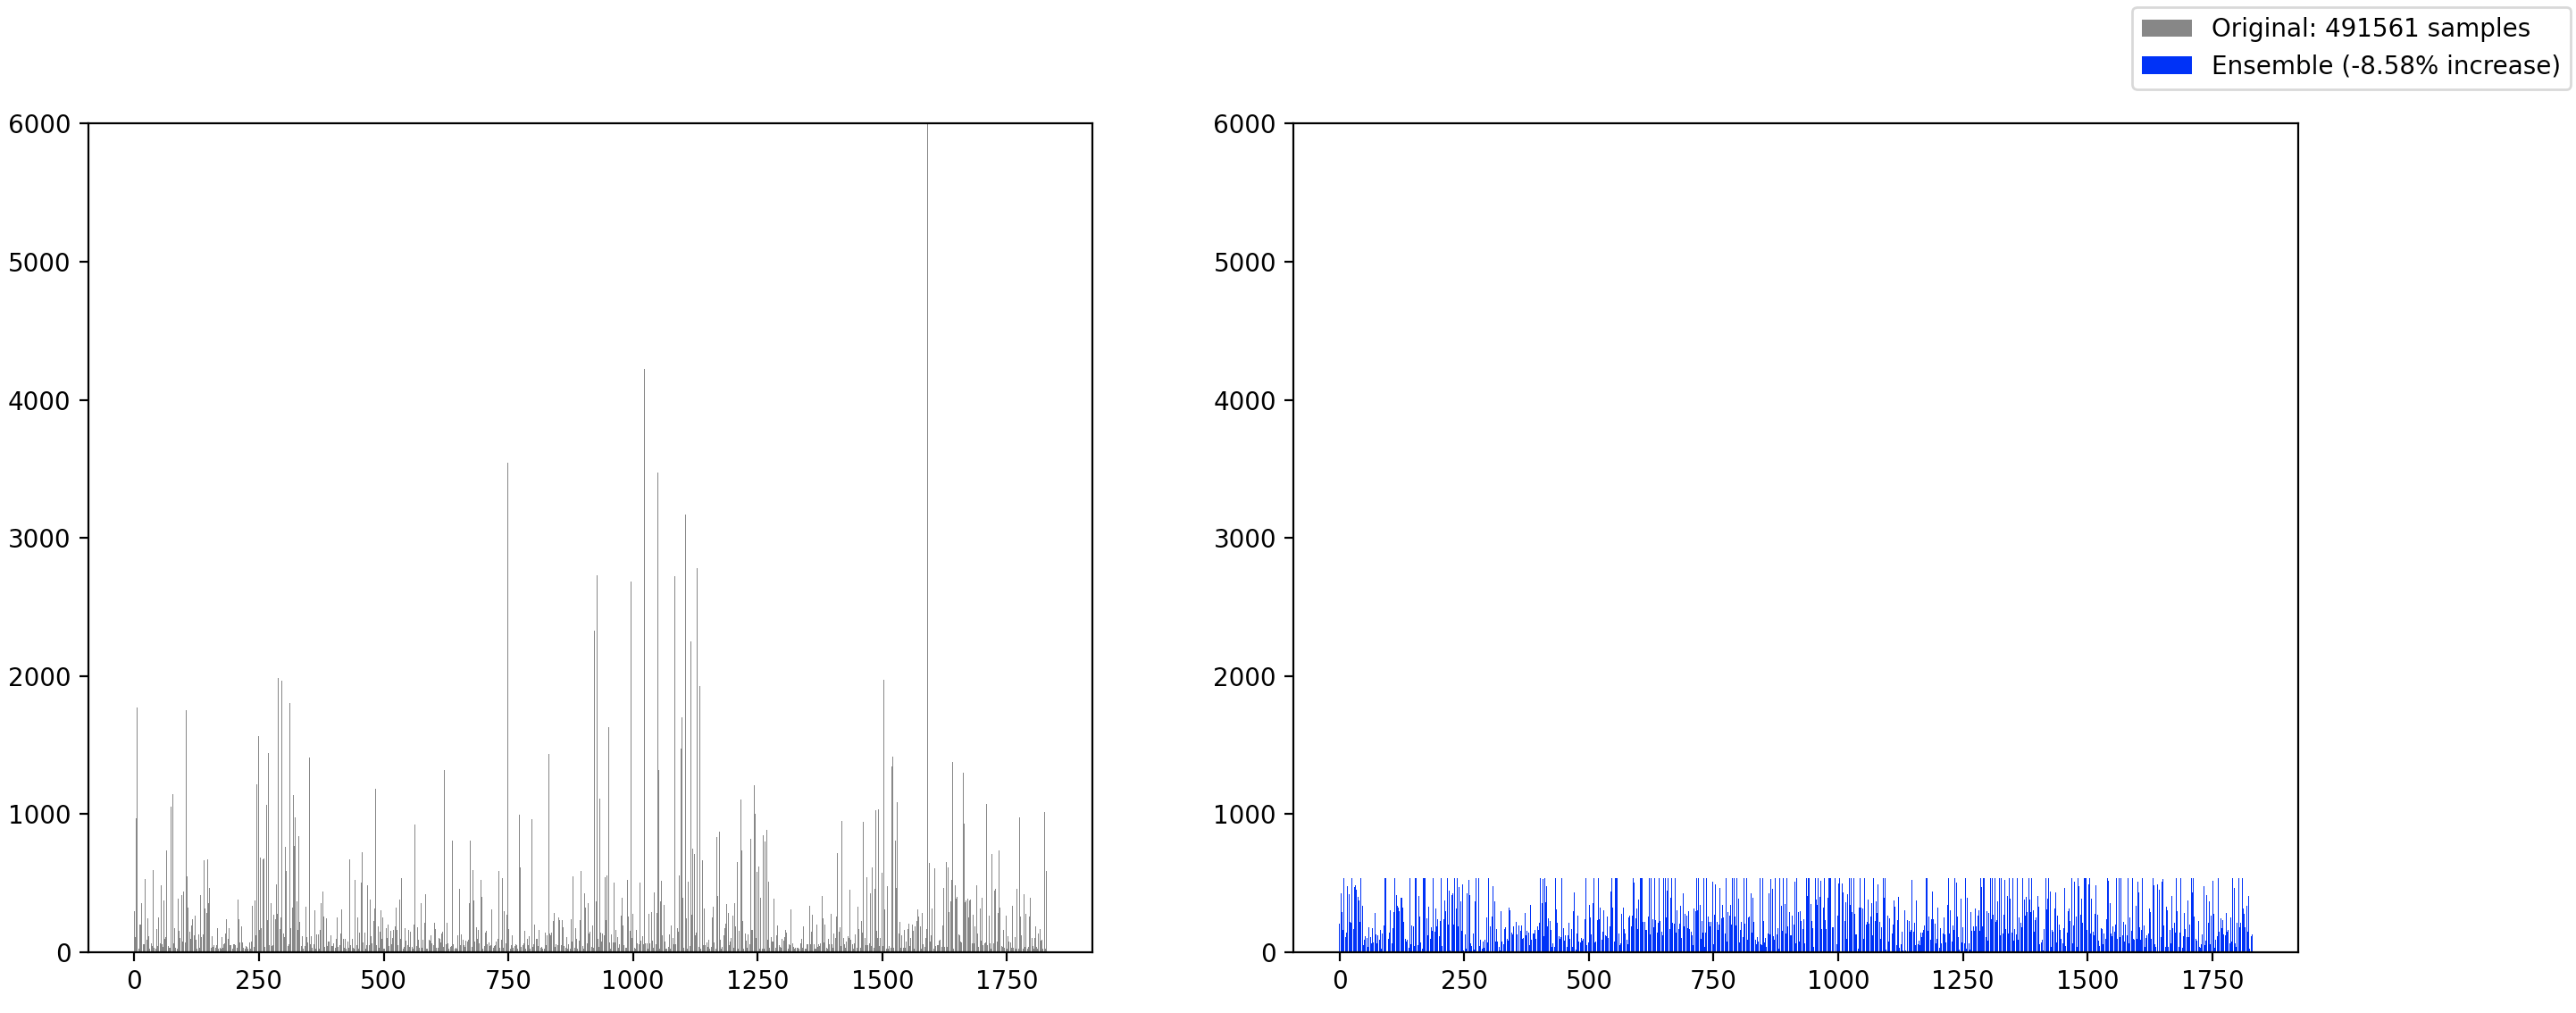
\includegraphics[width=1.0\textwidth]{figures/imbalance/ensemble}
    \caption{Final ensemble sampling method (right) compared to original dataset (left) where the final ensemble produces a dataset similar in size to that of the original.}
    \label{fig:ensemble_sampler}
\end{figure}

\section{Model training and prediction performance}

After the training dataset was constructed, encoded, and balanced, the model was trained using different approaches as described in \cref{sec:training_process}. This section describes the results from the training processes, the final approach used, and the resulting model's performance and predictions resulting from the evaluation process described in \cref{sec:evaluation_process}.

\subsection{Training process}

As described in \cref{sec:training_process}, multiple training processes were evaluated in order to find the most appropriate method of training a larger model on an extensive dataset. For the \acrfull{xgb} model, three different training processes were evaluated in this process.

First, the iterative approach was evaluated by training the model in batches of \textit{600 000} samples at the time. This approach seemed to work as intended, however, it was discovered that during subsequent training batches, the performance of the model dropped off for each iteration. It seemed as if the model did not handle continuous training of the same model as well as it does when training one model from scratch using the complete dataset. Furthermore, the parameter \textit{``early\_stopping\_rounds''} was used in the other approaches as a method of telling the model to stop training if it does not see any improvements after the given number of rounds. When this parameter is set using the iterative approach, the model can stop producing new trees before it has constructed the total number of trees allowed by the \textit{``n\_estimators''} parameter. Since the first iteration can produce a model with less trees than allowed, the next iteration fails as the number of allowed trees does not match with the previous model's actual number of trees. Although there are ways around this issue, as using the early stopping rounds parameter is useful to avoid overfitting, the iterative approach did not seem the most appropriate during the development process.

Next, it was attempted to train the model using the external memory, or ``out-of-core'' memory version of \acrshort{xgb}. In this approach, the \acrshort{xgb} library is provided a \textit{libsvm} file which it converts to an optimized matrix format which is kept on the computers file system. However, all attempts at training the model using external memory were unsuccessful as the training process consumed all of the running computer's available memory and resulted in a ``bad allocation`` memory error. There seems to either be a misconfiguration or an underlying issue with the Python library used in the implementation. However, since the expected results from this approach should be the same as training the model in one iteration on a capable computer, these issues were not further looked into, although, it could be beneficial to reduce the resource requirements for the training process for future use. Therefore, it could warrant more investigation for future work.

Finally, the entire dataset was used to train the final model in one iteration on a computer capable of running the process. The training process ran over the course of two days and consistently required around 200GB of memory. The vast memory consumption could be somewhat reduced by not evaluating the model during the training process which is appropriate for future training processes after the model has been trained and the training configuration has been validated. As described in \cref{sec:training_process}, an extra copy of the training and test datasets were kept in memory to continuously evaluate and monitor the training process.

\subsection{Performance}

During the training process, the performance of the model was continuously evaluated to measure logarithmic loss and multi-class classification error. \cref{fig:eval_set} shows these metrics plotted over each boosting round in the training process. Both graphs starts converging at 100 decision trees have been constructed at around \textbf{1.5} log loss, and around \textbf{0.3} classification error. This corresponds to around \textbf{70\%} accuracy. Since the graphs have not completely converged, it is possible to either increase the learning rate parameter or increase the number of estimators in the tree, although it seems as if the graphs are very close to converging, so it might not increase performance noticeably and increases risk of overfitting. As there is very little difference between the performance on the training set and evaluation set, it indicates that the model is not overfitting, however, it might indicate that the model is over optimistic. This could occur when there are several similar samples in the training and the test datasets and could be a consequence of the sampling techniques used to balance the dataset.

\begin{figure}[htbp]
    \centering
    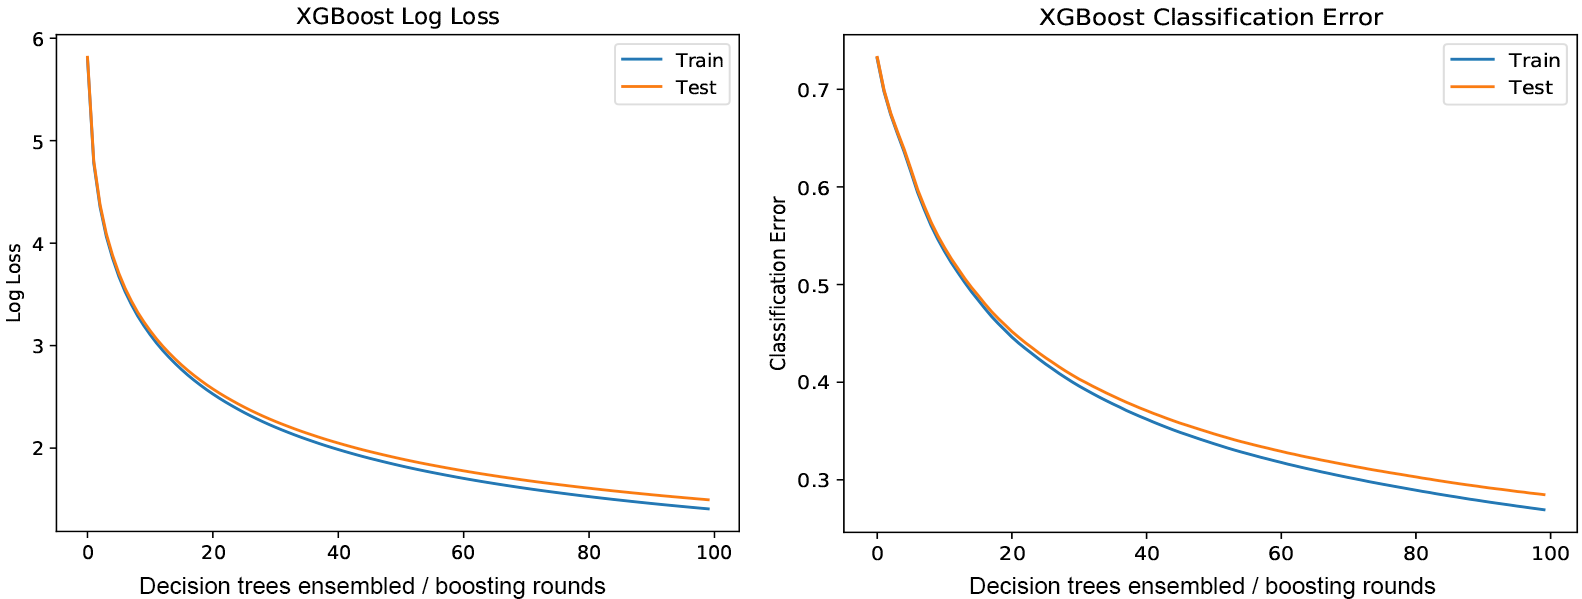
\includegraphics[width=1.0\textwidth]{figures/results/eval_set}
    \caption{Logarithmic loss and classification error metrics tracked per boosting round in the training process.}
    \label{fig:eval_set}
\end{figure}

After the training process finished, the test dataset was used to make predictions to further evaluate the results. From the resulting predictions, accuracy was calculated to be \textbf{72\%}, and a class report was generated that shows more metrics for each possible class, or encoded arrival port, that might provide more insight into the model's performance than accuracy. \cref{lst:class_report} shows a summarized output from this class report showing the metrics precision, recall, f1-score, and support for each class as well as the aggregated mean values from all of the classes. As mentioned in \cref{sec:model_evaluation}, f1-score is based on precision and recall and is particularly appropriate for measuring performance on imbalanced datasets, and as \cref{lst:class_report} shows, the f1-score does not deviate much from the estimated accuracy of \textbf{72\%}, or \textbf{0.72}. This indicates that the accuracy value is reliable and is not biased by dataset imbalance.

\begin{lstlisting}[
    caption={Class report based on prediction results from the test dataset. The performance of the classifier is evaluated per class by using precition, recall, f1-score, and support.},
    label=lst:class_report,
    showstringspaces=false,
    basicstyle=\ttfamily,
]
[XGBoostClassifier] Class Report:
             precision    recall  f1-score   support      pred
0             0.378049  0.240310  0.293839     258.0     164.0
1             0.816850  0.810909  0.813869     275.0     273.0
2             0.722222  0.541667  0.619048     312.0     234.0
3             0.672727  0.377551  0.483660     294.0     165.0
...           ...       ...       ...          ...       ...
3067          0.824675  0.849498  0.836903     299.0     308.0
3068          0.833922  0.778878  0.805461     303.0     283.0
3069          0.773050  0.762238  0.767606     286.0     282.0
3070          0.614035  0.557325  0.584307     314.0     285.0
...           ...       ...       ...          ...       ...
avg / total   0.718698  0.715150  0.712737  878049.0  878049.0

\end{lstlisting}

Lastly, in order to ensure the model is not overfitted, a three-fold cross validation process was employed. \cref{lst:cv_result} shows the results from the three folds that the model was trained on. It is recommended, or common to use more folds ranging from five to 10, however, because of the long training time and time limitations, only three folds were used. As described in \cref{sec:model_evaluation}, since the standard deviation (noted as ``std. dev.'' in \cref{lst:cv_result}) is low, the model is likely to not be overfitted.

\begin{lstlisting}[
    caption={Output from 3-fold cross validation. \todo{update numbers}},
    label=lst:cv_result,
    showstringspaces=false,
    basicstyle=\ttfamily,
]
 Folds:      [0.70569399 0.71297481 0.72244745]
 Mean:       0.7137054183485277
 Std. dev.:  0.006859056778768982
\end{lstlisting}

\section{Prediction results}

After the model was trained and evaluated, \textit{20\%} of the total training dataset was used to evaluate the model. This evaluation process resulted in around \textit{880 000} example predictions. These predictions were further analyzed to discuss the impact and meaning of the different features used in the dataset. These results are presented in this section.

\subsection{Feature importances}

An added benefit of using a tree based model such as the \acrfull{xgb} or \acrfull{rf} model is that they can provide insight into the importances of features, or attributes. In a decision tree based ensemble, when constructing a tree, the training data is analyzed to find the best features to make splits, or branches, in the trees. After the training process, the models can then produce a ranking over what features best divided the dataset best. This is referred to as feature importance.

\begin{table}[htbp]
    \centering
    \begin{tabularx}{0.6\textwidth}{X X}
        \bfseries{Feature} & \bfseries{Importance} \\ \toprule
        sspd\_mstd         & 0.443659 \\ \midrule
        departure\_port    & 0.226288 \\ \midrule
        segmentation       & 0.180907 \\ \midrule
        sspd\_dist         & 0.083816 \\ \midrule
        trajectory\_length & 0.065331 \\ \bottomrule
    \end{tabularx}
    \caption{Feature importances based on the \acrshort{xgb} decision tree ensemble process}\label{tab:feature_importances}
\end{table}

\cref{tab:feature_importances} shows an overview of the produced feature importances after the \acrshort{xgb} training process. As it shows, the most important feature was the \acrshort{mstd} value at a ranking of 0.44 out of 1.0, followed by the vessel's departure port, segmentation value, and then the similarity value and voyage length. This analysis can further help decide if features are worth dropping from the dataset, and insight into what attributes are good indicators during voyage predictions. As mentioned in \cref{sec:dataset_imbalance}, the attributes ``segment'', and ``sub-segment'' were combined into one segmentation value in order to ensure that no invalid segment and sub-segment combinations could be generated by sampling methods. A disadvantage of this is that the feature importances of the two attributes are lost in favor of the combined value. However, from test runs made during the development process with and without sampling, the importance of segment and sub-segment were usually ranked where segmentation is in \cref{tab:feature_importances} with sub-segment being more important than segment.

Furthermore, the results from test dataset predictions were analyzed to find the impact of the attributes that mostly served as weights for the \acrshort{mstd} value, namely, the similarity value (\textit{sspd\_dist}) and trajectory length. \cref{lst:dist_length_impact} shows an output from the evaluation process which shows that the distance value was smaller, on average, for correct predictions while trajectory length did not considerably differ from correct and incorrect predictions. It makes sense that the distance, or similarity, value is lower for correct predictions as the more similar the most similar historical trajectory is, the more valuable the \acrshort{mstd} value is. For instance, if a voyage's most similar historical trajectory has a \textit{sspd\_dist} of 0, it is following an exact path of a previous voyage. In this case, the similarity value for correct predictions was on average around \textit{43\%} lower than for incorrect predictions. For the trajectory length, it would make sense that the longer the voyage had traveled, the easier it would be to predict its destination, thus, the length should be longer for correct predictions. However, this is not the case for these predictions. This could be explained by the fact that shorter voyages might be easier to predict than long voyages for small vessels. For instance, it is presumable that, passenger vessels with very short but frequent trajectories are very easy to predict thus bringing the average length down for correct predictions. To confirm this hypothesis, further investigation into the specific segments and sub-segments is required.

\begin{lstlisting}[
    caption={Mean values of similarity value and trajectory length for correct and incorrect predictions.},
    label=lst:dist_length_impact,
    showstringspaces=false,
    tabsize=1,
    basicstyle=\ttfamily,
]
mean ssp_dist for correct predictions:           115642.48170757179
mean trajectory_length for correct predictions:  17.662729492637958

mean ssp_dist for erroneus predictions:           201713.174255885
mean trajectory_length for erroneus predictions:  18.841843522761508
\end{lstlisting}

\subsection{Segment predictability}

As it relates to research question 2 (\cref{sec:research_questions}), the \textit{880 000} predictions from the test dataset were further analyzed in search of patterns in predictability of different types of vessels. These results also serves to gain further insight into the value of the performance metrics. \cref{fig:segment_accuracy} shows a bar chart of the initial accuracy of predictions per segment, and it shows that there are some differences in accuracy per segment overall, but the most of the segments have a similar level of predictability. For example, vessels of the segment ``other'' were the easiest to predict and had the highest accuracy of \textit{76\%}. This is likely to be caused by different types of passenger vessels that lie within this segment. These vessels produce many predictable voyages as they travel between a few number of ports with a high frequency. Furthermore, the ``other'' segment also include very specialized vessels that are limited in terms of possible destination ports.

\begin{figure}[htbp]
    \centering
    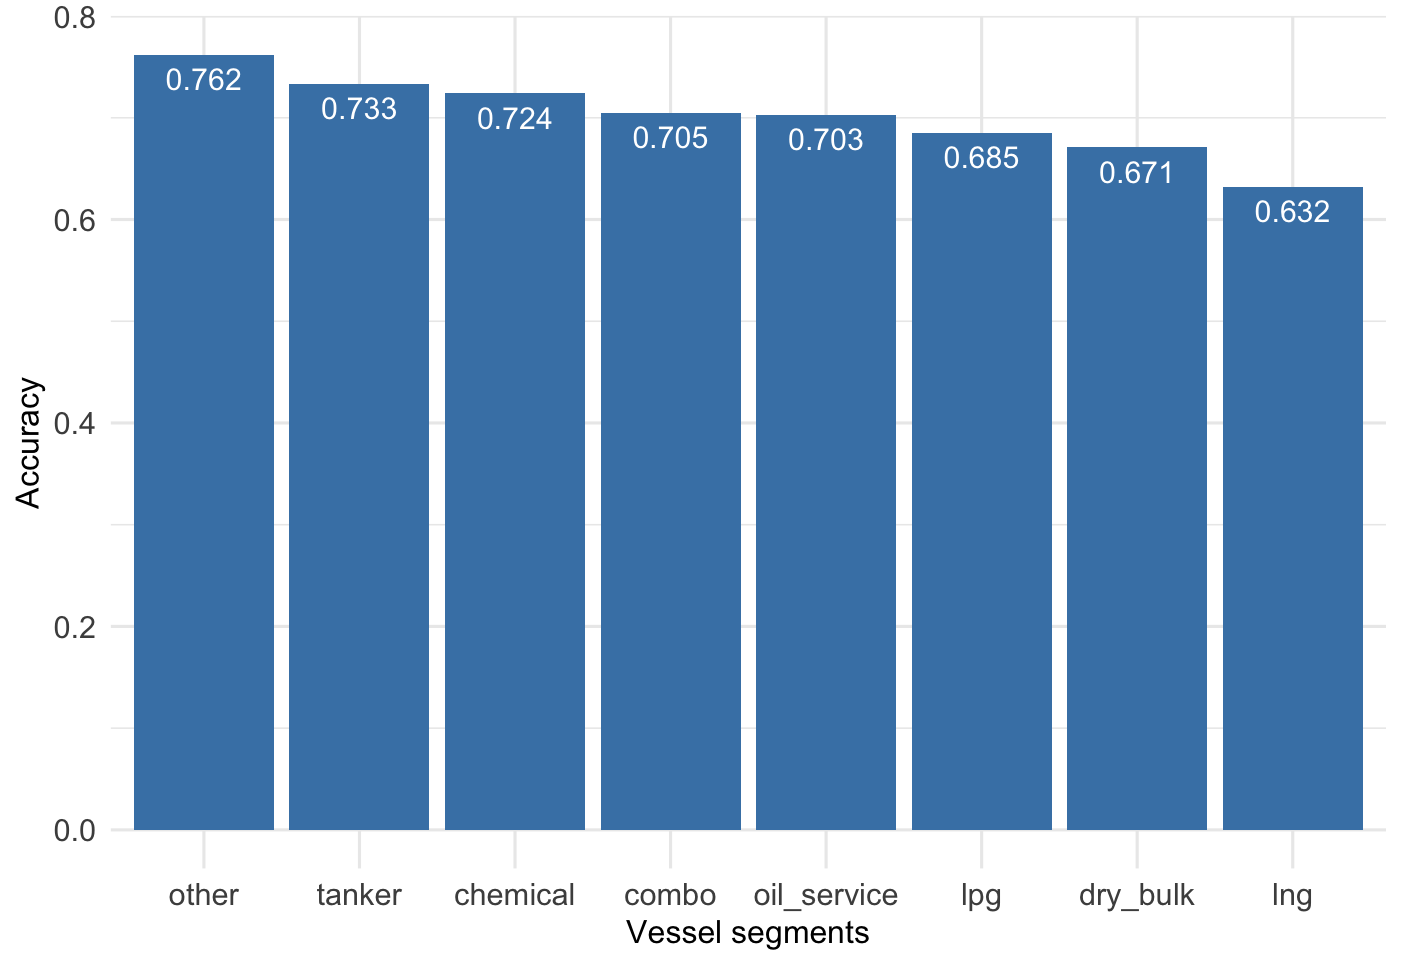
\includegraphics[width=0.8\textwidth]{figures/results/segment_accuracy_new}
    \caption{Accuracy of predictions from test set per segment.}
    \label{fig:segment_accuracy}
\end{figure}

As \cref{fig:other_accuracy} shows, and as expected, the accuracy of the passenger related sub-segments were very high. Since these are so high in frequency and has shorter trajectories, they may be the main cause that the average trajectory length was lower for correct predictions than incorrect ones. On the other hand, container and car ``roll on/roll off'' (roro) vessels travel longer distances less frequently but were also quite predictable. Another segment that could affect the average trajectory length and similarity values for correct predictions is the oil service segment. The oil service vessels should be easy to predict as these vessels travel to oil platforms and often back to the same or another nearby port. However, for these vessels, their trajectories would have been harder to consider as they often do not use the ``moored'' AIS navigational status when arriving at oil platforms. This can lead to very long trajectories that are hard to compare to others, therefore, these vessels should rely more on the departure port rather than the \acrshort{mstd} related values. In general, the ``other'' and ``oil service'' segments are not very relevant for \acrfull{mo}'s customers or for bigger actors in the industry, however, some sub-segments such as container and other general cargo ships can be quite relevant.

\begin{figure}[htbp]
    \centering
    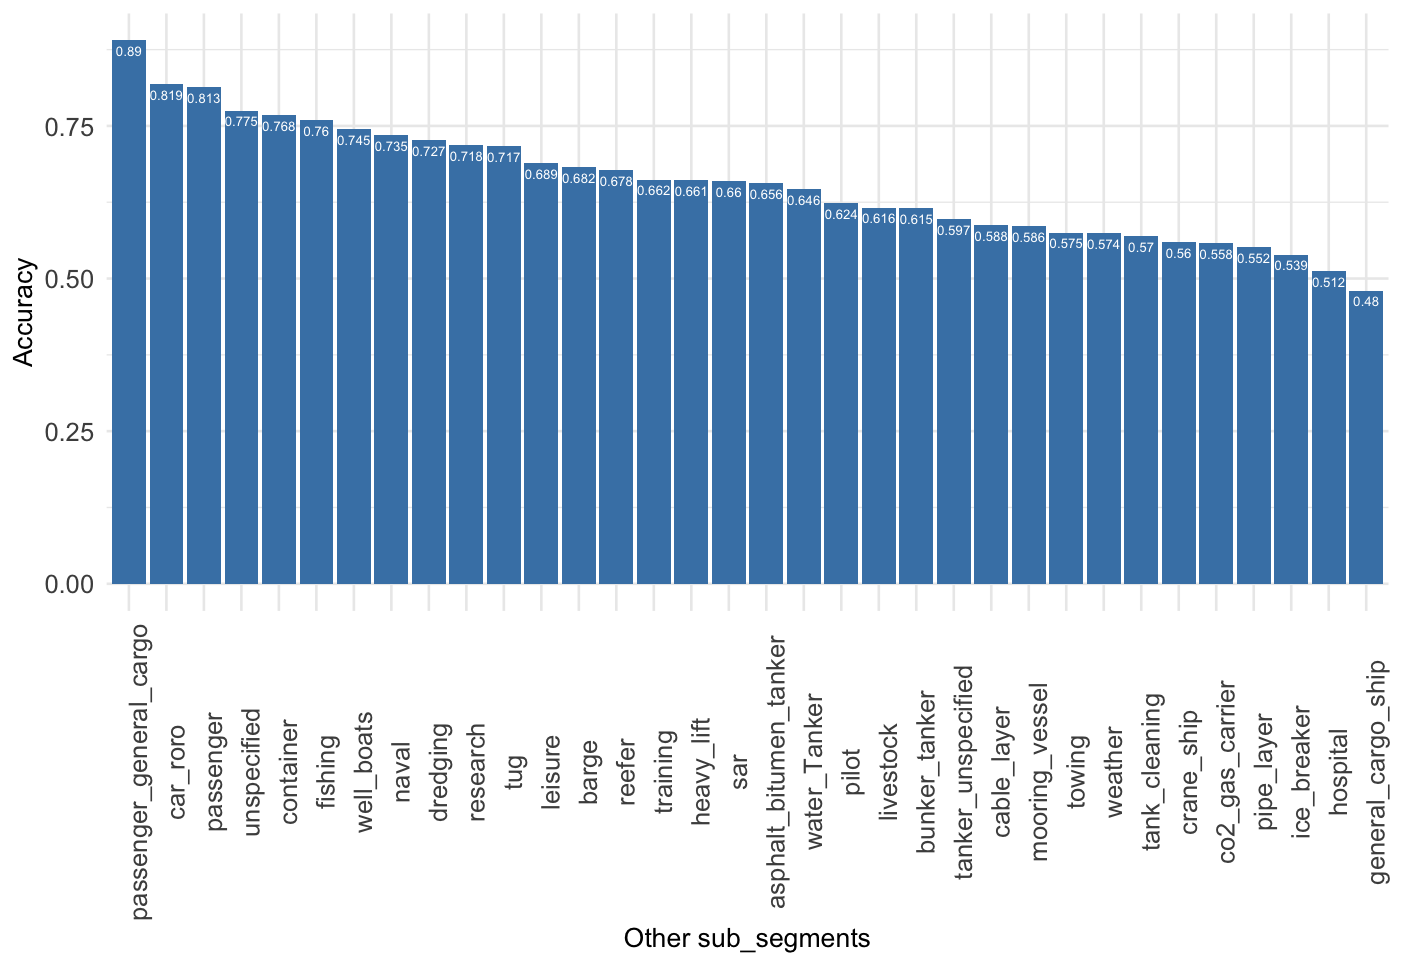
\includegraphics[width=1.0\textwidth]{figures/results/seg_other_acc}
    \caption{Accuracy of predictions per sub-segment within the ``other'' segment.}
    \label{fig:other_accuracy}
\end{figure}
\begin{figure}[htbp]
    \centering
    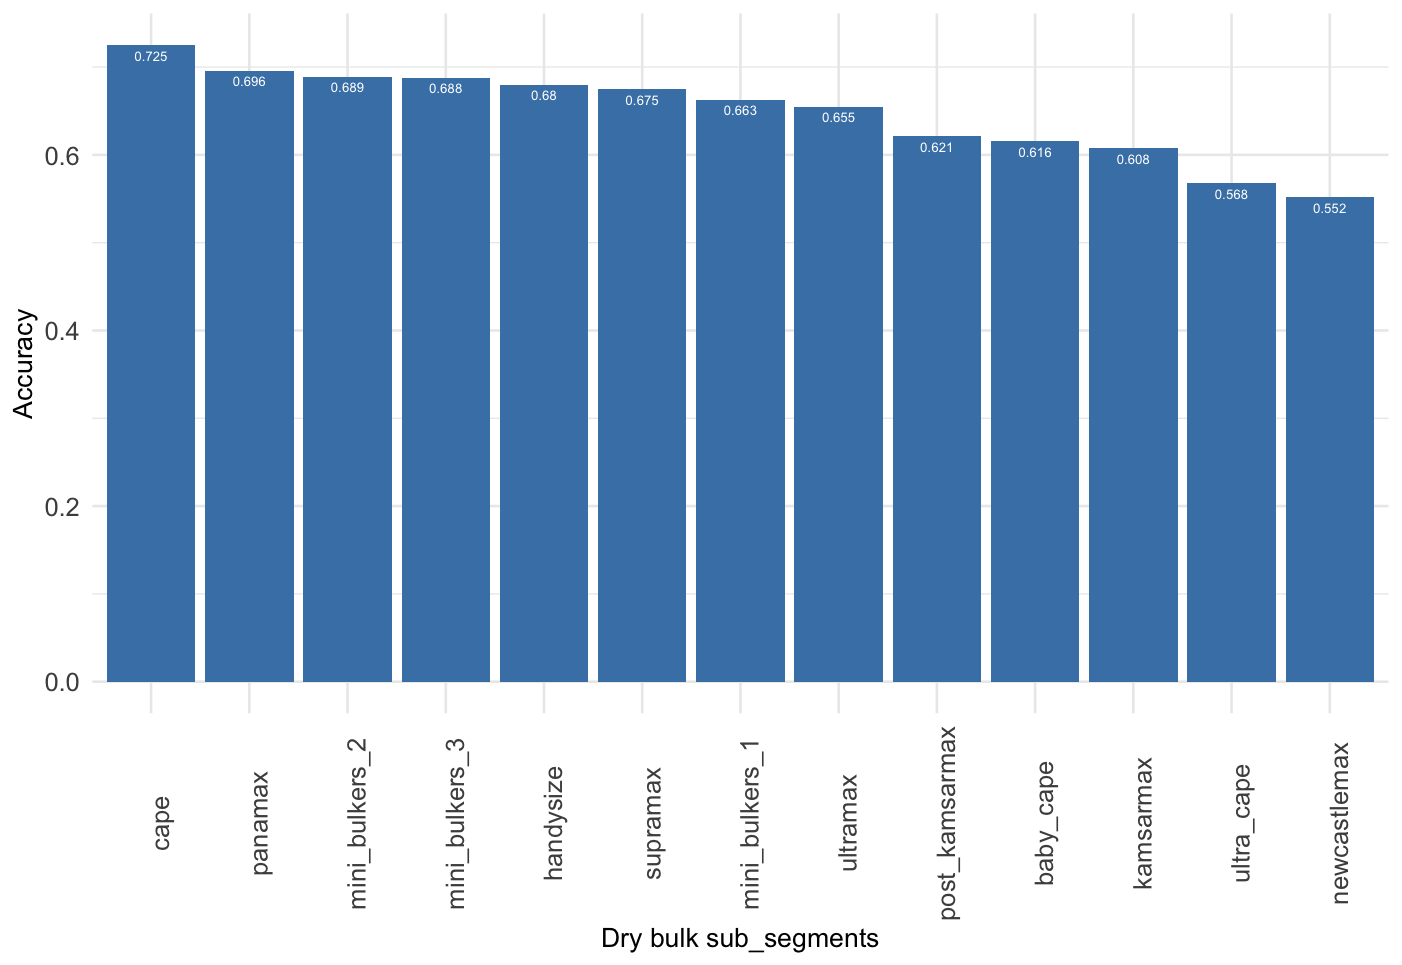
\includegraphics[width=0.8\textwidth]{figures/results/seg_dry_bulk_acc}
    \caption{Accuracy of predictions per sub-segment within the ``dry\_bulk'' segment.}
    \label{fig:dry_bulk_accuracy}
\end{figure}


The dry bulk cargo industry, on the other hand, has more commercial interest. \cref{fig:dry_bulk_accuracy} shows the accuracy per sub-segment for the dry bulk cargo segment. The dry bulk sub-segments are based on the vessels' cargo capacities and sizes, however, as \cref{fig:dry_bulk_accuracy} shows, there seems to be little correlation between vessel size and accuracy. The two most accurately predicted sub-segments are large vessels, however, they are followed closely by the smaller sub-segments, and the two least predictable types are some of the largest. Thus, the uniqueness of the sub-segment value itself had more impact on predictions than the implied size and capacity of the vessels.

\begin{figure}[htbp]
    \centering
    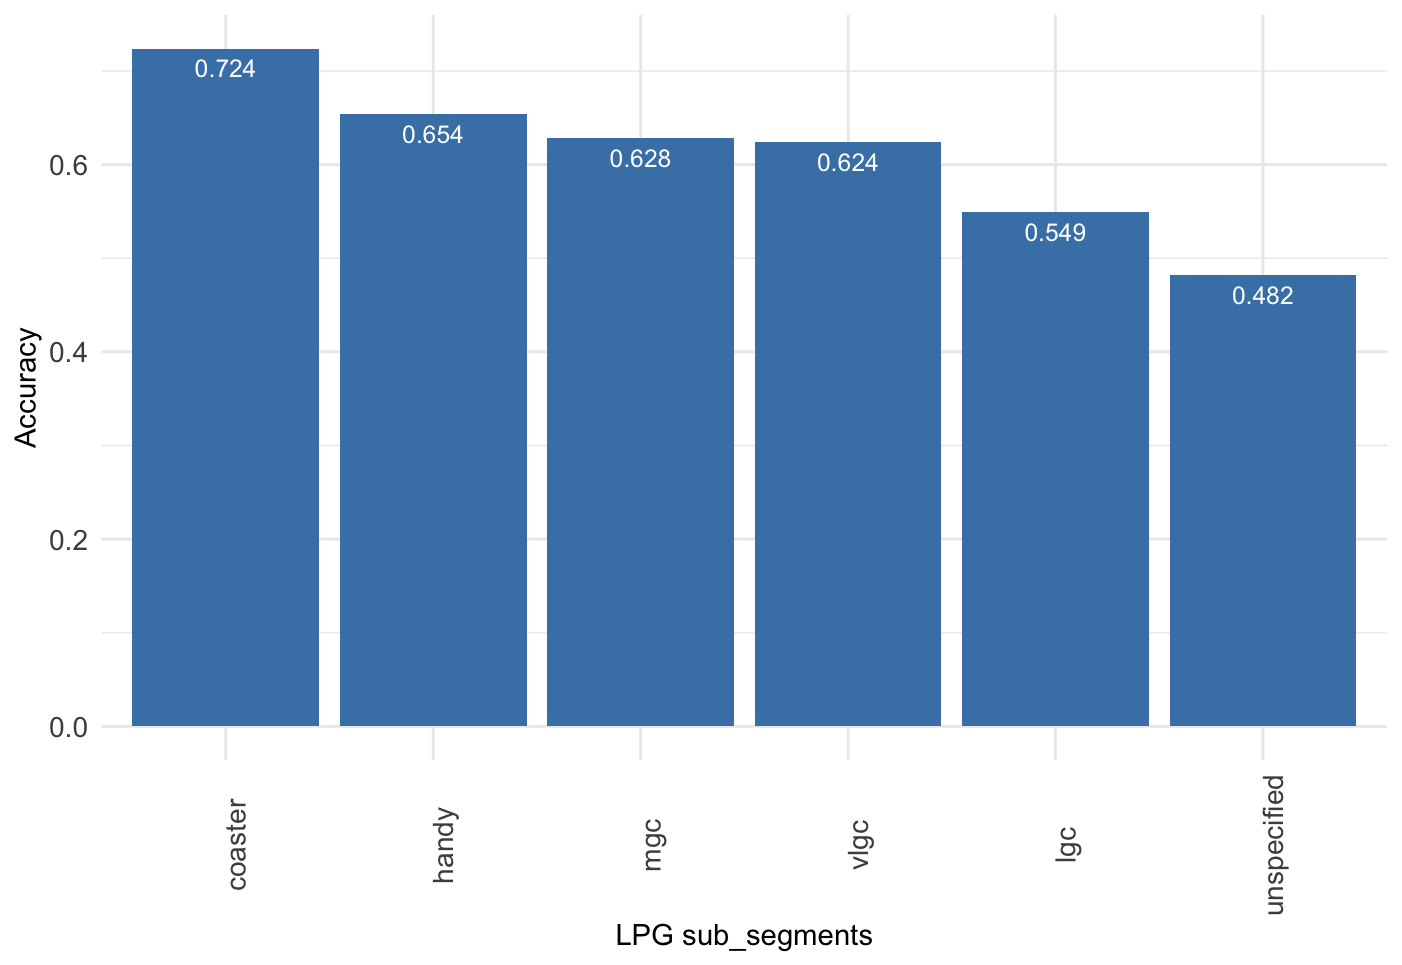
\includegraphics[width=0.9\textwidth]{figures/results/seg_lpg_acc}
    \caption{Accuracy of predictions per sub-segment within the ``LPG'' segment.}
    \label{fig:lpg_accuracy}
\end{figure}

The prediction results for tanker sub-segments show similar results as to the dry bulk ones, however, some other segments does seem to show that size and capacity indeed might be correlated to predictability in different ways. For instance, in the chemical segment the two largest sub-segments have the highest accuracies of \textit{90\%} and \textit{85\%}, however, the remaining sub-segments does not show much difference correlated to size. There seem to be a slight correlation in chemical vessels that show that larger vessels are easier to predict than smaller ones, however, for other segments the opposite correlation seems to occur. The \acrfull{lng} and \acrfull{lpg} vessels have the highest correlation between size and accuracy, but in the opposite direction compared to the chemical vessels. \cref{fig:lpg_accuracy} shows that the three smallest \acrshort{lpg} sub-segments \textit{coaster}, \textit{handy}, and \textit{MGC} have the highest accuracy, while the two largest sub-segments \textit{VLGC} and \textit{LGC}  have lower accuracies. This is similar to that of the \acrshort{lng} vessels (\cref{fig:lng_accuracy}) where the largest sub-segments \textit{QMax}, and \textit{QFlex} are harder to predict than the smaller sub-segments.

\begin{figure}[htbp]
    \centering
    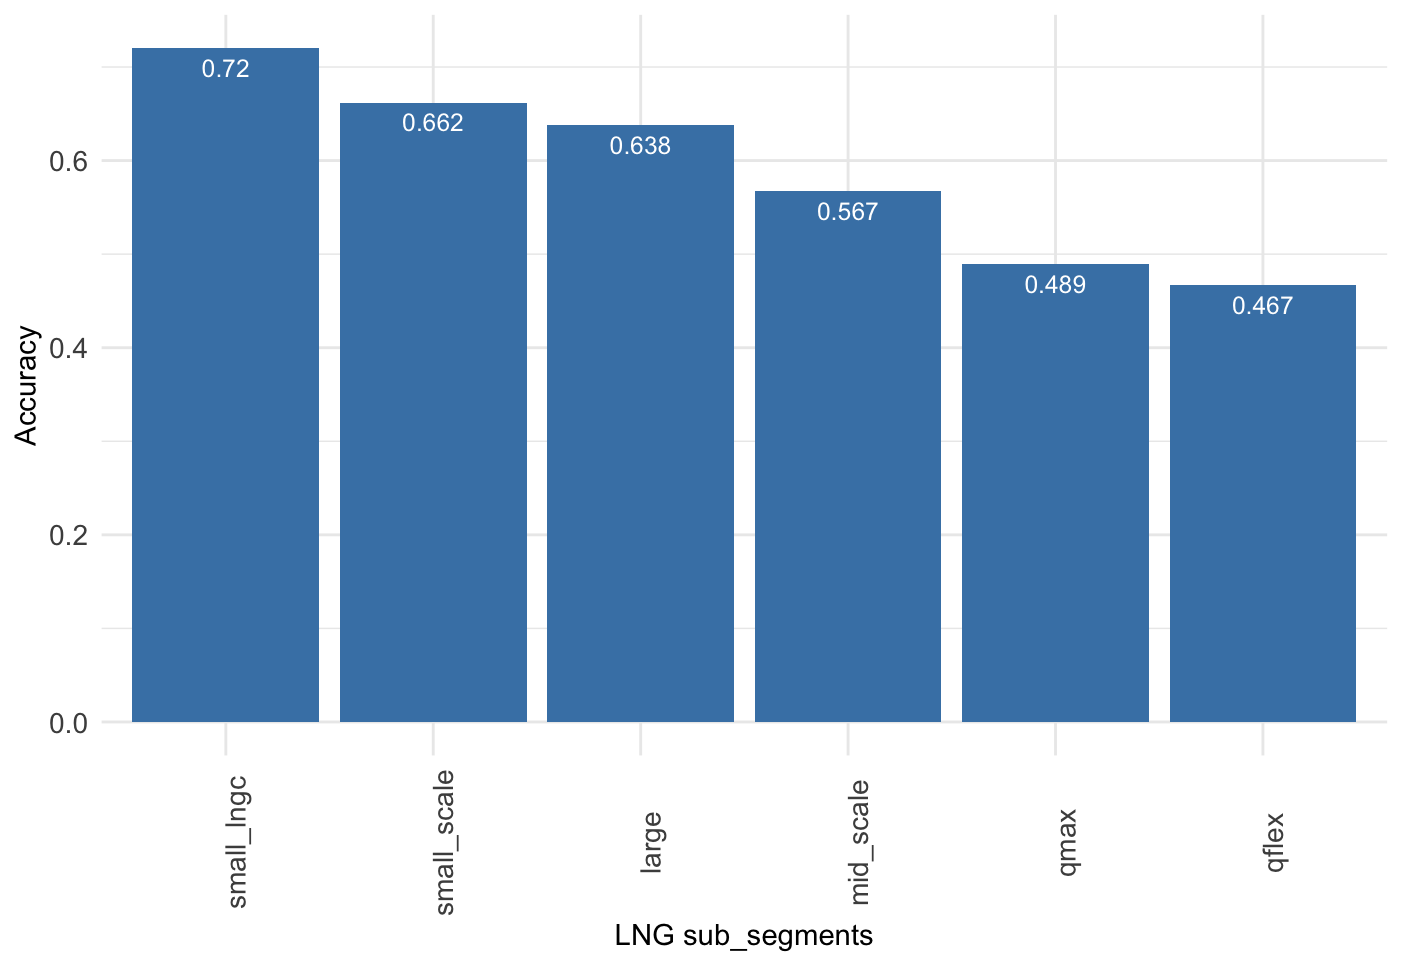
\includegraphics[width=0.9\textwidth]{figures/results/seg_lng_acc}
    \caption{Accuracy of predictions per sub-segment within the ``LNG'' segment.}
    \label{fig:lng_accuracy}
\end{figure}

Another interesting segment to analyze is the combo segment. These combination vessels can serve multiple functions in that they can carry different types of cargoes. In \cref{fig:segment_accuracy}, the combo segment showed a mid-range general accuracy level, however, when looking into the sub-segments, there are substantial differences in accuracies across the different types of combo vessels (\cref{fig:combo_accuracy}). The ``Klaveness Combination Carriers'' (CABU) and ``Oil-Bulk-Ore'' (OBO) vessels have the highest accuracies. However, there are only 12 CABU vessels and 5 OBO vessels in the world, or in \acrfull{mo}'s vessel database. On the other hand, there are 4700 chemical product tankers in the world that were also quite predictable. These vessels drive the general accuracy of the combo vessels up in \cref{fig:segment_accuracy} as the remaining sub-segments have substantially lower accuracies. It does, however, make sense that combo vessels are generally difficult to predict as they serve multiple functions which results in them having more possible destination ports they can load and unload at.

\begin{figure}[htbp]
    \centering
    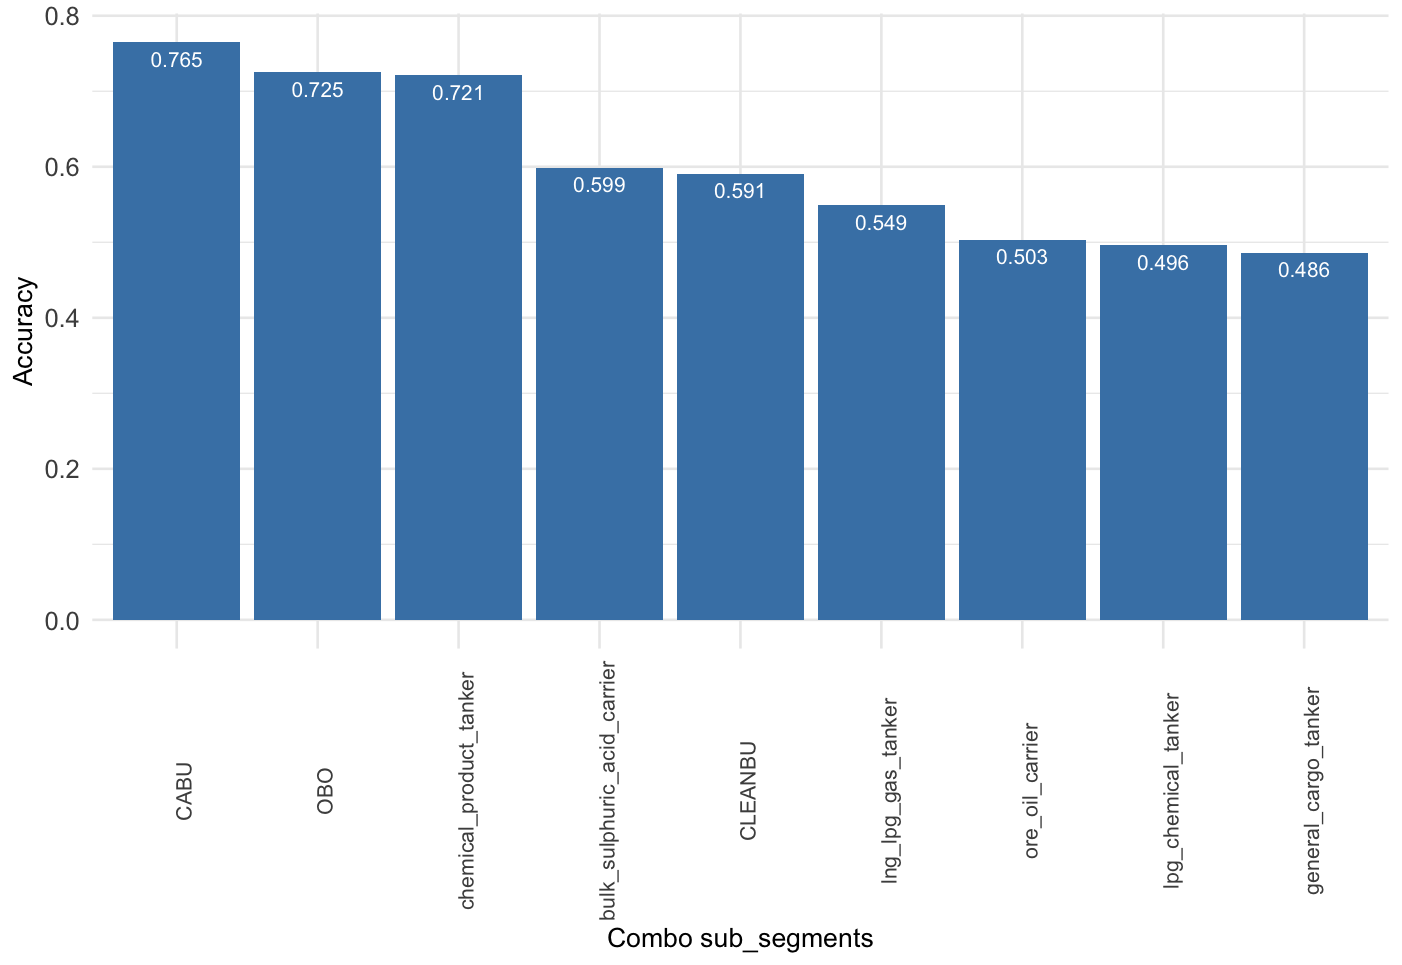
\includegraphics[width=0.9\textwidth]{figures/results/seg_combo_acc}
    \caption{Accuracy of predictions per sub-segment within the ``combo'' segment.}
    \label{fig:combo_accuracy}
\end{figure}

In regards to \texttt{RQ2} (\cref{sec:research_questions}), vessel segments and sub-segments seem to have a substantial impact on the predictability of vessels. As shown in \cref{tab:feature_importances}, the vessel segmentation had a feature importance close to that of the vessel's departure port. Furthermore, as discussed throughout this section, there are differences in accuracies for different segments and sub-segments, therefore, the vessel segmentation, with sub-segments in particular, had a significant impact on the predictions in the test dataset used during the evaluation process.

In regards to \texttt{RQ2a} the most predictable segment overall was the ``other'' segment (\cref{fig:segment_accuracy}). This was not entirely surprising as the sub-segments including passenger vessels are very predictable (\cref{fig:other_accuracy}). Moreover, the tanker, chemical, and combo vessels were similar in their accuracy levels, while \acrshort{lpg}, dry bulk, and \acrshort{lng} vessels were slightly less predictable. The sub-segment ``chemical product tanker'' drove the accuracy of the combo segment up to a similar level to that of the tanker and chemical vessels. This can be explained by the fact the this specific sub-segment has overlap into the two other segments. In other words, several tanker and chemical vessels are also present in the ``chemical product tanker'' combo sub-segment, so the accuracies is expected to be similar between the specific sub-segment and the tanker and chemical segments.

In response to \texttt{RQ2b}, and as mentioned earlier in this section, there seems to be some correlation between vessel size, capacity, and predictability, however, this only seems to be the case for some segments while for others, the uniqueness of the sub-segment value was the more important factor than the implied size or capacity. Thus, in regards to \texttt{RQ2b}, the prediction results does not conclusively indicate that larger vessels are more predictable than others.


\section{Applications and validity}

After the final training process, the resulting model is capable of predicting the future destination ports of traveling vessels. This section describes the intended usage and applications of the developed model as well as validation from experts in the industry.

\subsection{Usability}
\label{sec:usability}

As summarized in \cref{sec:pred_summary}, the process of predicting a single vessel's future destination port consists of first collecting the current traveling trajectory by fetching the positional \acrshort{ais} records from the last detected ``moored'' navigational status was transmitted to the last transmitted position. This trajectory must then be simplified as described in \cref{sec:trajectory_sampling}, then the \acrfull{mstd} of the must be calculated using the \acrshort{sspd} method with the traveling trajectory and every other historical trajectory departing the same port. The vessel's \acrshort{mstd}, segmentation, the distance returned from the \acrshort{sspd} method, and the length of the trajectory can be used to predict the vessel's next destination. The final trained model is saved to a file so it can quickly be loaded when making predictions. Thus, a program can be written that reads the trained model, receives an outgoing voyage, and predicts its next destination port.

In regards to re-training the model with new data, two approaches can be used. The simplest but more time consuming approach is to completely retrain the model after a substantial amount of new data is available. The training process takes around two days to complete using all of the historical dataset using a capable computer. Another approach could be to use \acrfull{xgb}'s support for iterative, or continuous learning as described in \cref{sec:training_process}. After the training process has completed, the \acrshort{xgb} model can be saved to file for future evaluation and predictions.

Finally, since the proposed solution can predict vessel's future destination ports, it could also be applied to forecast the availability of vessels. By providing the model with the current trajectories of all traveling vessels in the world, the model's output would indicate how many vessels of different segments will be positioned at different ports around the world. Given a method for estimating the time taken for each vessel to reach their predicted destination port, the model can be used to indicate what vessels will be positioned at a port in a given time interval. The model itself has no aspect of time, or \acrshort{eta}, however, there are existing methods and tools available today that can estimate how long it takes for vessels to travel between ports such as established distance tables\footnote{\url{https://sea-distances.org/}} or routing estimators. For instance, \acrfull{mo} offers a routing estimator to their customers that is capable of finding the shortest path between any given two positions across the seas. The proposed solution could therefore be integrated with this tool to forecast the supply of vessels at different ports in a given time interval.

\subsection{Expert validation}

Furthermore, in order to establish the validity of the proposed solution from a commercial perspective, a select number of shipping experts were interviewed in order to establish the validity of the process taken and the final results. These commercial actors were contacted via the collaborative company \acrfull{mo} who has a substantial network in the shipping industry. The commercial actors were presented with the proposed solution as well as the steps taken throughout the development process and asked questions in a semi-structured manner in order to gain insight into their perspective on the following topics:

\begin{itemize}
    \item Existing methods used to obtain predictions of vessel positions or vessel availability.
    \item Aspects of the thesis' solution that may prove to be valuable, and areas to improve before commercial consideration.
    \item Validity of the proposed voyage definition and possible alternative approaches.
    \item The impact of vessel segmentation and possible other information that could provide more insight into vessels' voyage patterns thus improving predictions.
\end{itemize}

The commercial actors interviewed works at high positions at different shipping related companies in Norway with many years of experience in the field. In respect to their privacy, their names, positions, or related companies will not be disclosed in this thesis, only a summary of the obtained information is presented.

\subsubsection{Existing methods of obtaining information}

One interviewee explained they did not use many digital tools in their decision making processes. They had been using \acrfull{mo} to gain some overview, but mostly relied on non-digital methods of obtaining information. It was clear the source considered the most reliable was information and analysis provided by shipping brokers. These brokers provides information and predictions regarding the relevant segment's market, cargo, and vessel supply. It was also clear that information provided by any digital solution would require extensive testing and validation before it could be considered as any form of replacement or addition to information provided by trusted brokers. It was also suggested that a tools such as proposed in this thesis would probably have high value for the brokers themselves, to aid in their information gathering processes.

\subsubsection{Valuable aspects of the proposed solution, and areas of improvement}

From the imagined usability described in \cref{sec:usability}, the aspect of obtaining a forecast of vessel supply in different ports and regions seemed to be the most promising aspect of the thesis from a commercial perspective. The interviewees explained that the aspect of cargo supply is, to some degree, quite predictable as the production of different supplies are quite cyclic and there are many detectable factors that indicate ebbs and flows in productions. Since the areas of high cargo supply are known, knowing how many competing vessels are available in these areas could be valuable information in that it would help the actors decide whether to focus on certain cargoes in the different areas or not. However, the interviewee expressed some skepticism of the quality of such as solution as it was thought that an immense amount of data would be required to make accurate predictions, and further expressed the need for extensive testing and validation before it would be considered valuable to them. It was also expressed that it was of no interest to them of knowing of vessels of segments other than their fleet, and suggested that a model specially trained for their segment would probably be of higher value to them.

\subsubsection{Validity of the proposed voyage definition}

The chosen vessel voyage definition was explained and the example described in \cref{sec:results_voyage_definition} was presented to the interviewees for their evaluation. Based on their response, it seemed that the suggested voyage definition would be a technically correct solution as it is based on the vessels themselves expressing via \acrshort{ais} that they are moored at different ports. However, another promising approach was suggested by one of the commercial actors. They suggested that the navigational status could be ignored if additional port information were to be used. For instance, when vessels stop at loading ports, they are likely to load, or depart, and at known unloading ports, the visiting vessels are likely to unload, or arrive. This could be implemented by using additional port information in combination with the clustering approach described in \cref{sec:clustering}. An imagined issue with this approach, however, was that some bunkering ports also serve other functions such as unloading, therefore, it could be more difficult to separate bunkering visits from unloading activities. This approach seems promising, however, it requires additional port information to know if they are loading, unloading, or bunkering ports.


\subsubsection{Additional vessel, or voyage information for prediction improvement}

Lastly, the interviewees were asked what vessel or voyage features they imagined could gain insight into voyage patterns and subsequently improving destination predictions. In addition to the vessels' segment and sub-segment they thought that the loading condition of the vessels would have a substantial impact on predictions. For example, if a vessel is loaded, it has fewer possible destination ports as it must arrive at an unloading port to unload. On the other hand, if the vessel is unloaded, or in ballast condition, it will probably visit a loading port next. It is possible to estimate a vessel's loading condition by looking at the vessel's current draft in static \acrshort{ais} messages. The draft of a vessel describes how deep the vessel is traveling, in meters, in the water. This value is higher when the vessel carries cargo, and lower if it is in ballast. Thus, if the information regarding vessels' loaded conditions were known during a voyage, the model could easily be trained to recognize these patterns and most likely be more accurate. Moreover, it was suggested that ports' depth restrictions could be considered when making predictions. As the current draft, or depth of the vessel is known, it can only arrive at ports that is deep enough to receive it. For instance, for larger vessels, there are fewer ports that has the capability of receiving them than small vessels. Lastly, other factors such as the current season, or month, could also have an impact on predictions as voyages are quite cyclic in nature, especially for some cargoes such as grain which is harvested at certain times of year at different locations in the world.
